\chapter{Description of the situation (rich picture and forbilleder)}\fxnote{Dette chapter skal måske rykkes. Kan vi følge SU struktur fra slides!!!!!!!}

\section{Rich Picture}
Figure \ref{RigtBillede} shows a Rich picture. This rich picture gives an overview of the users situation from the viewers position. The symbols represent different units, processes and problems. To begin with we will look at the symbols and explain them. Afterwards the situation will be explained in depth.

  \begin{figure}[H]
	\centering
	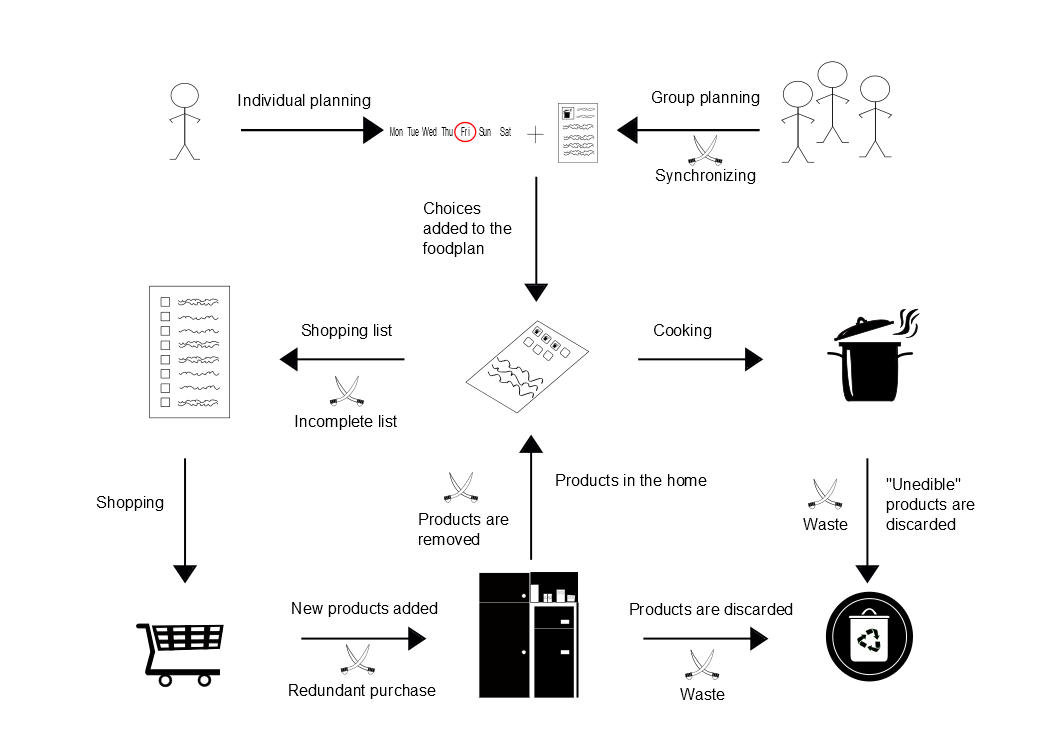
\includegraphics[width=1.00\textwidth]{Grafik/FoodPlanner/InkscapeTegninger/RigtBillede.png}
	\caption{A rich picture of the user's situation from the viewers position}
	\label{RigtBillede}
\end{figure}

\textbf{Units} includes people, physical objects, organizations and roles. On the top line there are the \textsf{stick man} symbol which is used to represent a user and then there are the \textsf{group of users} symbol. On the middle line there the \textsf{overview of the food plan} symbol and \textsf{shopping list} symbol which is used to depict the user's overview of the two units. On the bottom line there are the \textsf{inventory} symbol used to depict the household's storage of food products and the \textsf{trashcan} symbol.    
\fxnote{er det okay at figurens symboler får en anden font end resten af den tilhørende tekst??}
\textbf{Processes} includes different categories such as work and production, planning and control and information treatment.     
cooking, shopping, planning

\textbf{Problems}
syncing, list, cooking, product remove, waste, purchase, 

Figure \ref{RigtBillede} can also be divided into different context areas. The areas represent contexts in which different symbols are performed most often. The contexts are in the home and out of the home. Some symbols can belong in both contexts such as planning your meals which includes the user symbols, day + recipe and food plan\fxnote{hed det food plan?} overview symbols.       